\documentclass{article}
\usepackage{graphicx}
\usepackage{tikz}
\textheight=25.5cm \textwidth=18cm \topmargin=-1.8cm%
\evensidemargin=-0.8cm \oddsidemargin-0.8cm%

\begin{document}

\begin{center}
{\large Dissection Puzzles}
\end{center}

1. Cut each of these shapes into two parts and build a square.

\tikzstyle{my help lines}=[gray,
thick,dashed]
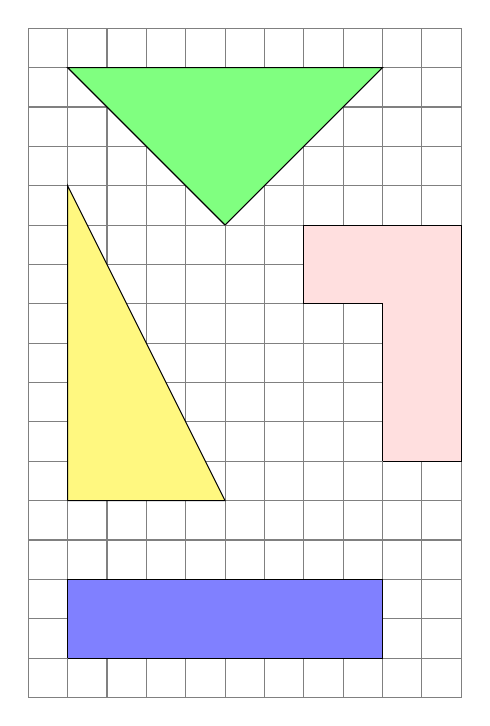
\begin{tikzpicture}
\draw[step=0.5cm,color=gray] (0,0) grid (5.5,8.5);
\draw[step=0.5cm,fill=blue!50] (0.5, 0.5) -- (4.5, 0.5) -- (4.5, 1.5) -- (0.5, 1.5) -- (0.5, 0.5);
\draw[step=0.5cm,fill=yellow!50] (0.5, 2.5) -- (2.5, 2.5) -- (0.5, 6.5) -- (0.5, 2.5);
\draw[step=0.5cm,fill=pink!50] (4.5, 3) -- (5.5, 3) -- (5.5, 6) -- (3.5, 6) -- (3.5, 5) -- (4.5, 5) -- (4.5, 3);
\draw[step=0.5cm,fill=green!50] (2.5, 6) -- (4.5, 8) -- (0.5, 8) -- (2.5, 6);
\end{tikzpicture}

\vspace{3mm}

2.

a) Cut a 6x4 rectangle into two parts, and build an 8x3 rectangle. Can you find two solutions?

b) Cut a 9x4 rectangle into two parts, and build a square.

c) Cut a 16x9 rectangle into two parts, and build a square.

\vspace{3mm}

3. Cut an arrow below into three parts, and build a 4x8 rectangle.

\tikzstyle{my help lines}=[gray,thick,dashed]
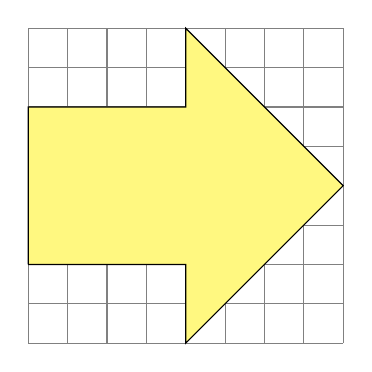
\begin{tikzpicture}
\draw[step=0.5cm,color=gray] (0,0) grid (4,4);
\draw[step=0.5cm,fill=yellow!50] (0, 1) -- (2, 1) -- (2, 0) -- (4, 2) -- (2, 4) -- (2, 3) -- (0, 3) -- (0, 1);
\end{tikzpicture}

\end{document}
